\section{Methodology}
	\subsection{Information Procurement}
	The main theme of the collected data would concentrate around the topic of internet sales platforms also known as E-Commerce. Several aspects make the topic beneficial for this research. Firstly, the very {\bfseries nature of E-Commerce}. By {\bfseries nature of E-Commerce} Platforms, I refer to the fact, that such companies are almost exclusively web-based. It is therefore probable that most of the company's marketing efforts as well as overall news relating to such a company, would circulate first and foremost in the Internet. Secondly, having all company-relevant news attainable foremostly from the web, means that such news would seep to social media faster in comparison to news, which are usually covered initially by traditional media such as television and Newspapers. 
	
		\subsubsection*{Search Terms}
		The data was collected in the form of relevant tweets from the {\bfseries Twitter Stream API}. A Tweet would be considered relevant if it contained a search parameter related contextually to E-Commerce. The initial efforts were concentrated around the web-store Amazon. Amazon appears to the most fruitful search parameter in terms of the quantity of tweets relating to it. Additional search words that were tested were {\bfseries Alibaba, Zalando} and {\bfseries Groupon}. 
		The widespread mention of Amazon in tweets is however somewhat over-inflated due to the extensive use of Amazon gift cards. Amazon gift-cards have become prominent due their variety of uses. A few examples of common practices involving Amazon gift cards are rewarding users for services, such as polls and questionnaires, enticing people to take part in events or groups, and being offered as general rewards in competitions and games. The plethora of uses, facilitates Amazon gift cards to be viewed as a sort of pseudo-currency in the internet. In turn this means, that Amazon could be mentioned in a Tweet, despite the context only indicating the Gift-card and being completely unassociated to the E-Commerce platform whatsoever.
		
		\subsubsection*{Collecting the Data}
		The gathering of Tweets was executed using a program written by me in the Python programming language. The main module being used in the program was a Twitter Streaming API called \textbf{Tweepy}. \textbf{Tweepy} is an open source interface, which allows communicating with the Twitters servers and sending queries requesting specific information from Twitter's databases. The interface allows for two main type of queries, \textbf{Rest} and \textbf{Streaming}. The former allows looking up information posted on Twitter in the past whereas the latter, as the name implies connects to an active data stream containing a narrowed down flow of tweets being actively published by Twitter users. Both types of API's are being offered for free to a certain extent, whereas almost unrestricted versions of the same API are offered as a proprietary fee-based product of Twitter. The free version of the \textbf{Rest API} is restricted to only looking up tweets posted in the last two to three weeks. And the gratis version of the \textbf{Streaming API} is restricted to a firehose narrowed down to about 15\% of the total Bandwidth of all current tweets.
		The tweets from the Twitter servers come in form of JSON strings, which allows for embedding other JSON objects in them, which allows for multi-level storage of Tweet properties. For example, one of the JSON objects integrated in each Tweet JSON object is the \textbf{USER} object for the tweet-poster. The \textbf{USER} object in turn contains all data publicly available in Twitter about a Twitter account such as, location, date of registration, homepage etc. An additional object of interest is the \textbf{ENTITIES} JSON object, which contains all outside references from the tweet's text such as, URLs, Multimedia, References to other tweets or other users. 
		This structure greatly eases the construction an analysis of a tweet and its features, since most of the necessary data is available from the tweet self and no further queries about the tweets and its posting-user are necessary.
		
		\subsubsection*{Data cleansing}
		It was observed that numerous tweets were being posted more than once and in some cases even hundreds of times. These similar tweets were using being posted by bots, as was evident from a short inspection of the user profile of the tweets poster. Evidently additional effort was being made by the programmers of the bots to try and mask the bot by slightly altering the content of the tweets. This was usually done by changing or adding characters which carry no meaning in themselves. Moreover, in furtherance of increasing the bots' credibility as an actual person, often times entire nets of such bot could be observed, wherein the bots would maintain friendship and following connections among themselves. This in turn, further adding to each of them having a multiplicity of friends and followers contributing to their veil of disguise as real human users of Tweeter.
		Several steps were made to try an avoid such bots. A passive precaution which was made, was marking users, which had posted tweets, the type of which was observed numerous times within the same query. The suspected users were added to a suspect database and were ignored in future queries. Another action made with the same purpose was a retrospective cleanup of the collected tweets, based on their content similarity. After closing a collection query, the tweets were scanned for having similar tweets and non-unique copies were filtered out. As a measure of similarity, the function \textbf{SequenceMatcher.ratio} from the \textbf{difflib} Python module was used {\color{red} \Large also try Levenshtein }. A round of cleanup using this procedure would usually reduce a data set by from one quarter and up to one half of its original size.
		
		\newpage
		
	\subsection{Building the Datasets}
	Once a list of labeled Tweets is obtained, the next stage is constructing a feature-set to be later passed on as input for training an ML Classifier. The features contained if the feature sets describe certain aspects and characteristics of a Tweet and its owner. Since Tweeters API provides a complete user profile incorporated inside the tweet itself, constructing features describing the user is done simultaneously to the features of the tweet itself.
	\\~\\
	{\LARGE \color{red}
		elaborate about stages of data collection:
	} \\ 
	{\color{red}
		1. Initial data: full of duplicates\\
		2. Filtered data - fewer duplicates and spam, but still rather very one-subject-centered. Leads to overfitting when classifying \\
		3. still untried - collect up to x (~400) tweets per day, for a duration of ~ 2 weeks
	}
		
		\subsubsection*{Types of Features}
		The features could be segregated into three distinctive groups. The first will be referred to as text-based features. As the name suggests, the features will mostly denote the presence or lack of specific characters such as emoticons and signs in the tweets text. Whether a tweet contains combinations or sequences of certain symbols as well as ratios defining the text also belong to this category.
		The second tier of features describe any special entities (Tweeter's nomenclature) contained within the tweet. Entities refer to non-textual contents of a tweet such as media (in form of pictures, sound or videos), URLs linking to external websites, Mentions or Retweets (Referring to other tweets or to tweeter profile pages) and finally Hashtags. A Hashtag is a word or phrase that starts with the symbol \textbf{\#} and that briefly indicates what a message (such as a tweet) is about \cite{dict_tweet}. Hashtags are used primarily to simplify looking up tweets or other social media messeges with a specific theme or content.
		
	\subsection{Training Classifier}	
	{\Large \color{red} ----- describe training, testing for confidence and splitting(called the holdout method) the df to train-test ----}
	\begin{figure}[h]
		
		\centering
		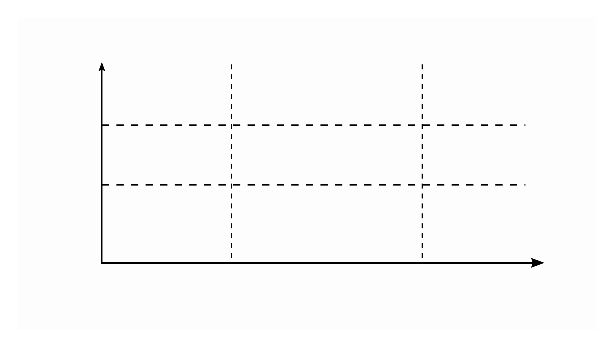
\includegraphics[width=0.5\textwidth]{methods}
		\caption{Clustering of Different Classifiers}
	\end{figure}

	\subsection{Classifier Types}
		{\color{red} \Large placeholder}
	
	
	
		
		
		
		